\documentclass[a4paper, 12pt]{article} % тип документа

%%%Библиотеки
%\usepackage[warn]{mathtext}	
\usepackage[T2A]{fontenc}   %Кодировка
\usepackage[utf8]{inputenc} %Кодировка исходного текста
\usepackage[english, russian]{babel} %Локализация и переносы
\usepackage{caption}
\usepackage{listings}
\usepackage{amsmath, amsfonts, amssymb, amsthm, mathtools}
\usepackage[warn]{mathtext}
\usepackage[mathscr]{eucal}
\usepackage{wasysym}
\usepackage{graphicx} %Вставка картинок правильная
\DeclareGraphicsExtensions{.pdf,.png,.jpg}
\graphicspath{ {images/} }

\setlength{\parskip}{0.5cm}

\usepackage{pgfplots}
\usepackage{indentfirst}
\usepackage{float}    %Плавающие картинки
\usepackage{wrapfig}  %Обтекание фигур (таблиц, картинок и прочего)
\usepackage{fancyhdr} %Загрузим пакет
\usepackage{lscape}
\usepackage{xcolor}
\usepackage[normalem]{ulem}
\usepackage{wasysym}
\usepackage{subfig}
\usepackage{graphicx}
\usepackage[ampersand]{easylist}


\usepackage{titlesec}
\titlelabel{\thetitle.\quad}

\usepackage{hyperref}
\newenvironment{comment}{}{}

%%%Конец библиотек

%%%Настройка ссылок
%%%	\hypersetup
%%%	{
%%%		colorlinks = true,
%%%		linkcolor  = blue,
%%%		filecolor  = magenta,
%%%		urlcolor   = blue
%%%	}
%%%Конец настройки ссылок


%%%Настройка колонтитулы
\pagestyle{fancy}
\fancyhead{}
\fancyhead[L]{1.1.4}
\fancyhead[R]{Апарин Сергей, группа Б01-205}
\fancyfoot[C]{\thepage}
%%%конец настройки колонтитулы


\usepackage[T2A]{fontenc}                        % кодировка
\usepackage[utf8]{inputenc}                        % кодировка исходного текста
\usepackage[english,russian]{babel}        % локализация и переносы
\usepackage{tikz}
\usepackage{pgfplots}

\begin{document}


%%%%\maketitle
%%%Начало титульника
\begin{titlepage}

    \newpage
    \begin{center}
        \normalsize Московский физико-технический институт \\(национальный исследовательский университет)
    \end{center}

    \vspace{6em}

    \begin{center}
        \Large Лабораторная работа по общему курсу физики\\
    \end{center}

    \vspace{1em}

    \begin{center}
        \Large \textbf{Отчёт о выполнении лабораторной работы 1.4.1\\ {Измерение интенсивности радиационного фона}}
    \end{center}

    \vspace{2em}

    \begin{center}
        \large Апарин Сергей Владимирович \\
        Группа Б01-205
    \end{center}

    \vspace{\fill}

    \begin{center}
        Долгопрудный \\2022
    \end{center}

\end{titlepage}
%%%Конец Титульника


%\\\\\\\\\\\\\\\\\\\\\\\\\\\\\\\\\\\\\\\\\\\\\\\\\\\\\\\\\\\\\\\\\\\\
\section* {1. Описание работы}


В работе измеряется интенсивность радиационного фона, в основном состоящего из потока космических частиц. Используются методы обработки полученных измерений при помощи построения графиков и их анализа.



Используемое оборудование:
\begin{itemize}
    \item счётчик Гейгера-Мюллера (СТС-6) для обнаружения космических лучей и измерения их интенсивности (по ионизации газа).
    \item компьютер с интерфейсом связи с счётчиком для считывания импульсов счётчика и фиксации результатов измерений.
    \item блок питания.
\end{itemize}


%\\\\\\\\\\\\\\\\\\\\\\\\\\\\\\\\\\\\\\\\\\\\\\\\\\\\\\\\\\\\\\\\\\\\\
\section* {2. Теоретические сведения и методика измерений}


Счётчик Гейгера-Мюллера представляет собой 2 электрода: катод - металлический цилиндр и анод - тонкая металлическая нить вдоль оси цилиндра.
Электроны, попадающие в счетчик ионизируют газ и разгоняются при напряжении 400 В, образуя с помощью конденсатора $C_1$ лавину электронов, которая создает импульс, передаваемый через конденсатор $C_2$ компьютеру.
Схема включения счётчика представлена на Рис. 1.


\begin{center}
    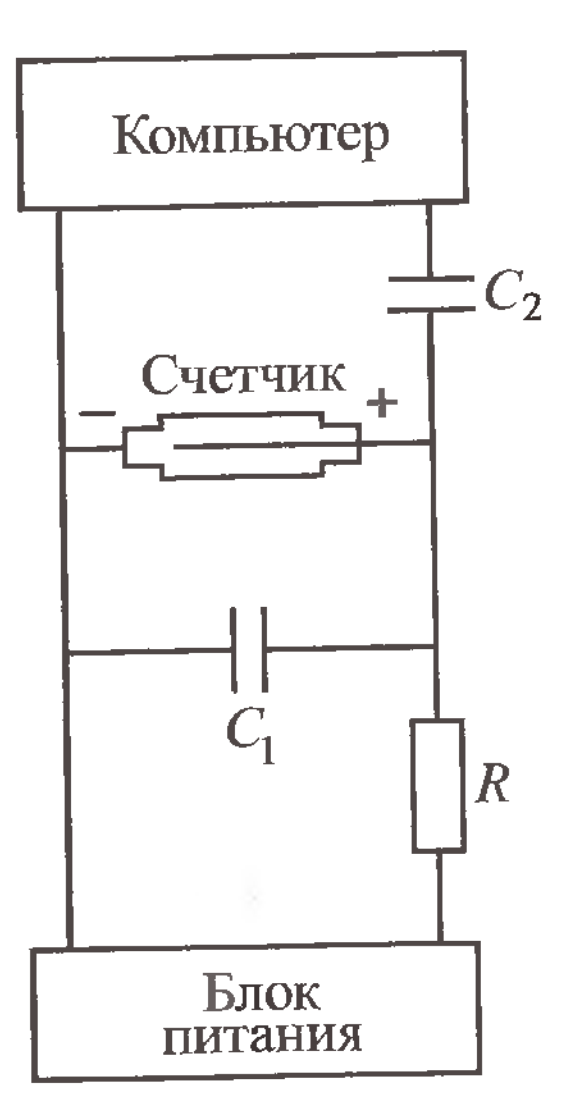
\includegraphics[width=4cm, height=7cm]{gayger.png}
\end{center}
\begin{center}
    {\scriptsize \textbf{Рис. 1} }
\end{center}


Методы обработки полученных результатов те же,что и для расчёта случайных погрешностей, так как в данном опыте измеряется величина, меняющаяся со временем случайным образом.


В процессе выполнения работы убеждаемся, что при увеличении числа измерений:

\begin{itemize}
    \item измеряемая величина флуктуирует.

    \item флуктуации среднего значения уменьшаются, а среднее занчение выходит на постоянну величину.

    \item флуктуации величины погрешности отдельного измерения уменьшаются, и погрешность отдельного эксперимента выходит на постоянну величину.

    \item флуктуации величины погрешности среднего значения уменьшаются, а сама величина убывает.

\end{itemize}



Будем использовать следующие формулы:

Среднее число срабатываний счетчика за одно измерение при проведении N измерений:
\begin{equation}
    \overline{n} = \frac{1}{N}\sum\limits_{i=1}^n n_i
\end{equation}


Среднеквадратичная ошибка отдельного измерения:
\begin{equation}
    \sigma_\text{отд} = \sqrt{\frac{1}{N}\sum\limits_{i=1}^n (n_i-\overline{n})^2}
\end{equation}


Определение стандартной ошибки величины $\overline{n}$:
\begin{equation}
    \sigma_{\overline{n}} = \frac{\sigma}{\sqrt{N}}
\end{equation}


И относительной ошибки:
\begin{equation}
    \epsilon_{\overline{n}} = \frac{\sigma_{\overline{n}}}{\overline{n}}
\end{equation}


Окончательный результат(оценка истинного среднего значения) будет соответствовать формуле:
\begin{equation}
    n_t = \overline{n} \pm \sigma_{\overline{n}}
\end{equation}



\section*{3. Результаты измерений и обработка данных}


\begin{table}[H]
    \centering
    \begin{tabular}{|l|l|l|l|l|l|l|l|l|l|l|}
        \hline
        № опыта & 1  & 2  & 3  & 4  & 5  & 6  & 7  & 8  & 9  & 10 \\ \hline
        0       & 27 & 23 & 26 & 23 & 21 & 22 & 13 & 35 & 31 & 24 \\ \hline
        10      & 28 & 19 & 30 & 19 & 19 & 32 & 29 & 25 & 30 & 22 \\ \hline
        20      & 27 & 29 & 32 & 30 & 30 & 23 & 21 & 32 & 25 & 24 \\ \hline
        30      & 31 & 21 & 28 & 26 & 24 & 35 & 31 & 28 & 35 & 27 \\ \hline
        40      & 22 & 28 & 28 & 29 & 24 & 24 & 32 & 25 & 27 & 30 \\ \hline
        50      & 27 & 17 & 21 & 22 & 17 & 25 & 32 & 26 & 33 & 20 \\ \hline
        60      & 15 & 22 & 21 & 24 & 31 & 26 & 10 & 24 & 23 & 17 \\ \hline
        70      & 16 & 25 & 27 & 27 & 22 & 27 & 35 & 26 & 28 & 16 \\ \hline
        80      & 29 & 25 & 25 & 23 & 26 & 23 & 27 & 21 & 20 & 23 \\ \hline
        90      & 23 & 26 & 21 & 24 & 35 & 19 & 18 & 30 & 25 & 34 \\ \hline
        100     & 32 & 31 & 23 & 24 & 22 & 24 & 29 & 30 & 38 & 24 \\ \hline
        110     & 16 & 30 & 27 & 13 & 22 & 29 & 28 & 25 & 24 & 27 \\ \hline
        120     & 16 & 24 & 22 & 28 & 22 & 26 & 16 & 29 & 23 & 25 \\ \hline
        130     & 23 & 25 & 17 & 31 & 26 & 25 & 27 & 25 & 26 & 30 \\ \hline
        140     & 26 & 27 & 22 & 25 & 26 & 20 & 28 & 23 & 30 & 22 \\ \hline
        150     & 28 & 27 & 27 & 31 & 33 & 25 & 27 & 20 & 31 & 30 \\ \hline
        160     & 24 & 22 & 31 & 24 & 23 & 16 & 20 & 13 & 26 & 22 \\ \hline
        170     & 23 & 30 & 29 & 26 & 20 & 17 & 25 & 28 & 26 & 13 \\ \hline
        180     & 31 & 31 & 25 & 26 & 30 & 23 & 18 & 25 & 30 & 34 \\ \hline
        190     & 31 & 21 & 19 & 30 & 22 & 24 & 26 & 27 & 33 & 30 \\ \hline
    \end{tabular}
    \begin{flushright}
        {\scriptsize \textbf{Таблица 1.}\\ \textbf {Число срабатываний счётчика за 20 с}}
    \end{flushright}
\end{table}

\begin{table}[H]
    \centering
    \begin{tabular}{|l|l|l|l|l|l|l|l|l|l|l|}
        \hline
        № опыта & 1  & 2  & 3  & 4  & 5  & 6  & 7  & 8  & 9  & 10 \\ \hline
        0       & 50 & 49 & 43 & 48 & 55 & 47 & 49 & 51 & 54 & 52 \\ \hline
        10      & 56 & 62 & 53 & 53 & 49 & 52 & 54 & 59 & 59 & 62 \\ \hline
        20      & 50 & 57 & 48 & 57 & 57 & 44 & 43 & 42 & 58 & 53 \\ \hline
        30      & 37 & 45 & 57 & 34 & 40 & 41 & 54 & 49 & 61 & 44 \\ \hline
        40      & 54 & 48 & 49 & 48 & 43 & 49 & 45 & 54 & 48 & 59 \\ \hline
        50      & 63 & 47 & 46 & 59 & 62 & 46 & 40 & 51 & 53 & 51 \\ \hline
        60      & 40 & 50 & 48 & 45 & 48 & 48 & 48 & 51 & 52 & 56 \\ \hline
        70      & 53 & 47 & 46 & 51 & 52 & 55 & 58 & 58 & 47 & 61 \\ \hline
        80      & 46 & 55 & 39 & 33 & 48 & 53 & 55 & 37 & 53 & 39 \\ \hline
        90      & 62 & 51 & 53 & 43 & 64 & 52 & 49 & 46 & 53 & 63 \\ \hline
    \end{tabular}
    \begin{flushright}
        {\scriptsize \textbf{Таблица 2.}\\ \textbf {Число срабатываний счётчика за 40 с}}
    \end{flushright}
\end{table}


\begin{table}[H]
    \centering
    \begin{tabular}{|l|l|l|l|l|l|l|l|}
        \hline
        Число импульсов $n_i$ & 4      & 5      & 6      & 7      & 8      & 9      & 10     \\ \hline
        Число случаев         & 4      & 0      & 10     & 16     & 22     & 29     & 28     \\ \hline
        Доля случаев $w_n$    & 0,01   & 0      & 0,025  & 0,04   & 0,055  & 0,0725 & 0,07   \\ \hline\hline
        Число импульсов $n_i$ & 11     & 12     & 13     & 14     & 15     & 16     & 17     \\ \hline
        Число случаев         & 39     & 47     & 48     & 42     & 27     & 28     & 27     \\ \hline
        Доля случаев $w_n$    & 0,0975 & 0,1175 & 0,12   & 0,105  & 0,0675 & 0,07   & 0,0675 \\ \hline\hline
        Число импульсов $n_i$ & 18     & 19     & 20     & 21     & 22     & 23     & 24     \\ \hline
        Число случаев         & 12     & 10     & 5      & 3      & 1      & 1      & 0      \\ \hline
        Доля случаев $w_n$    & 0,03   & 0,025  & 0,0125 & 0,0075 & 0,0025 & 0,0025 & 0      \\ \hline\hline
        Число импульсов $n_i$ & 25                                                           \\ \hline
        Число случаев         & 1                                                            \\ \hline
        Доля случаев $w_n$    & 0,0025                                                       \\ \hline
    \end{tabular}
    \begin{flushright}
        {\scriptsize \textbf{Таблица 3.}\\ \textbf {Данные для построения гистограммы распределения числа срабатываний счетчика за 10 с}}
    \end{flushright}
\end{table}


\begin{table}[H]
    \centering
    \begin{tabular}{|l|l|l|l|l|l|l|l|}
        \hline
        Число импульсов $n_i$ & 33   & 34   & 35   & 36   & 37   & 38   & 39   \\ \hline
        Число случаев         & 1    & 1    & 0    & 0    & 2    & 0    & 2    \\ \hline
        Доля случаев $w_n$    & 0,01 & 0,01 & 0    & 0    & 0,02 & 0    & 0,02 \\ \hline\hline
        Число импульсов $n_i$ & 40   & 41   & 42   & 43   & 44   & 45   & 46   \\ \hline
        Число случаев         & 3    & 1    & 1    & 4    & 2    & 3    & 5    \\ \hline
        Доля случаев $w_n$    & 0,03 & 0,01 & 0,01 & 0,04 & 0,02 & 0,03 & 0,05 \\ \hline\hline
        Число импульсов $n_i$ & 47   & 48   & 49   & 50   & 51   & 52   & 53   \\ \hline
        Число случаев         & 4    & 10   & 7    & 3    & 6    & 5    & 9    \\ \hline
        Доля случаев $w_n$    & 0,04 & 0,1  & 0,07 & 0,03 & 0,06 & 0,05 & 0.09 \\ \hline\hline
        Число импульсов $n_i$ & 54   & 55   & 56   & 57   & 58   & 59   & 60   \\ \hline
        Число случаев         & 5    & 4    & 2    & 4    & 3    & 4    & 0    \\ \hline
        Доля случаев $w_n$    & 0,05 & 0,04 & 0,02 & 0,04 & 0,03 & 0,04 & 0    \\ \hline\hline
        Число импульсов $n_i$ & 61   & 62   & 63   & 64                        \\ \hline
        Число случаев         & 2    & 4    & 2    & 1                         \\ \hline
        Доля случаев $w_n$    & 0,02 & 0,04 & 0,02 & 0,01                      \\ \hline
    \end{tabular}
    \begin{flushright}
        {\scriptsize \textbf{Таблица 4.}\\ \textbf {Данные для построения гистограммы распределения числа срабатываний счетчика за 40 с}}
    \end{flushright}
\end{table}


На основе данных из таблиц 3 и 4 построим гистаграммы распределения числа срабатываний счетчика за 10 с и 40 с:


\begin{center}
    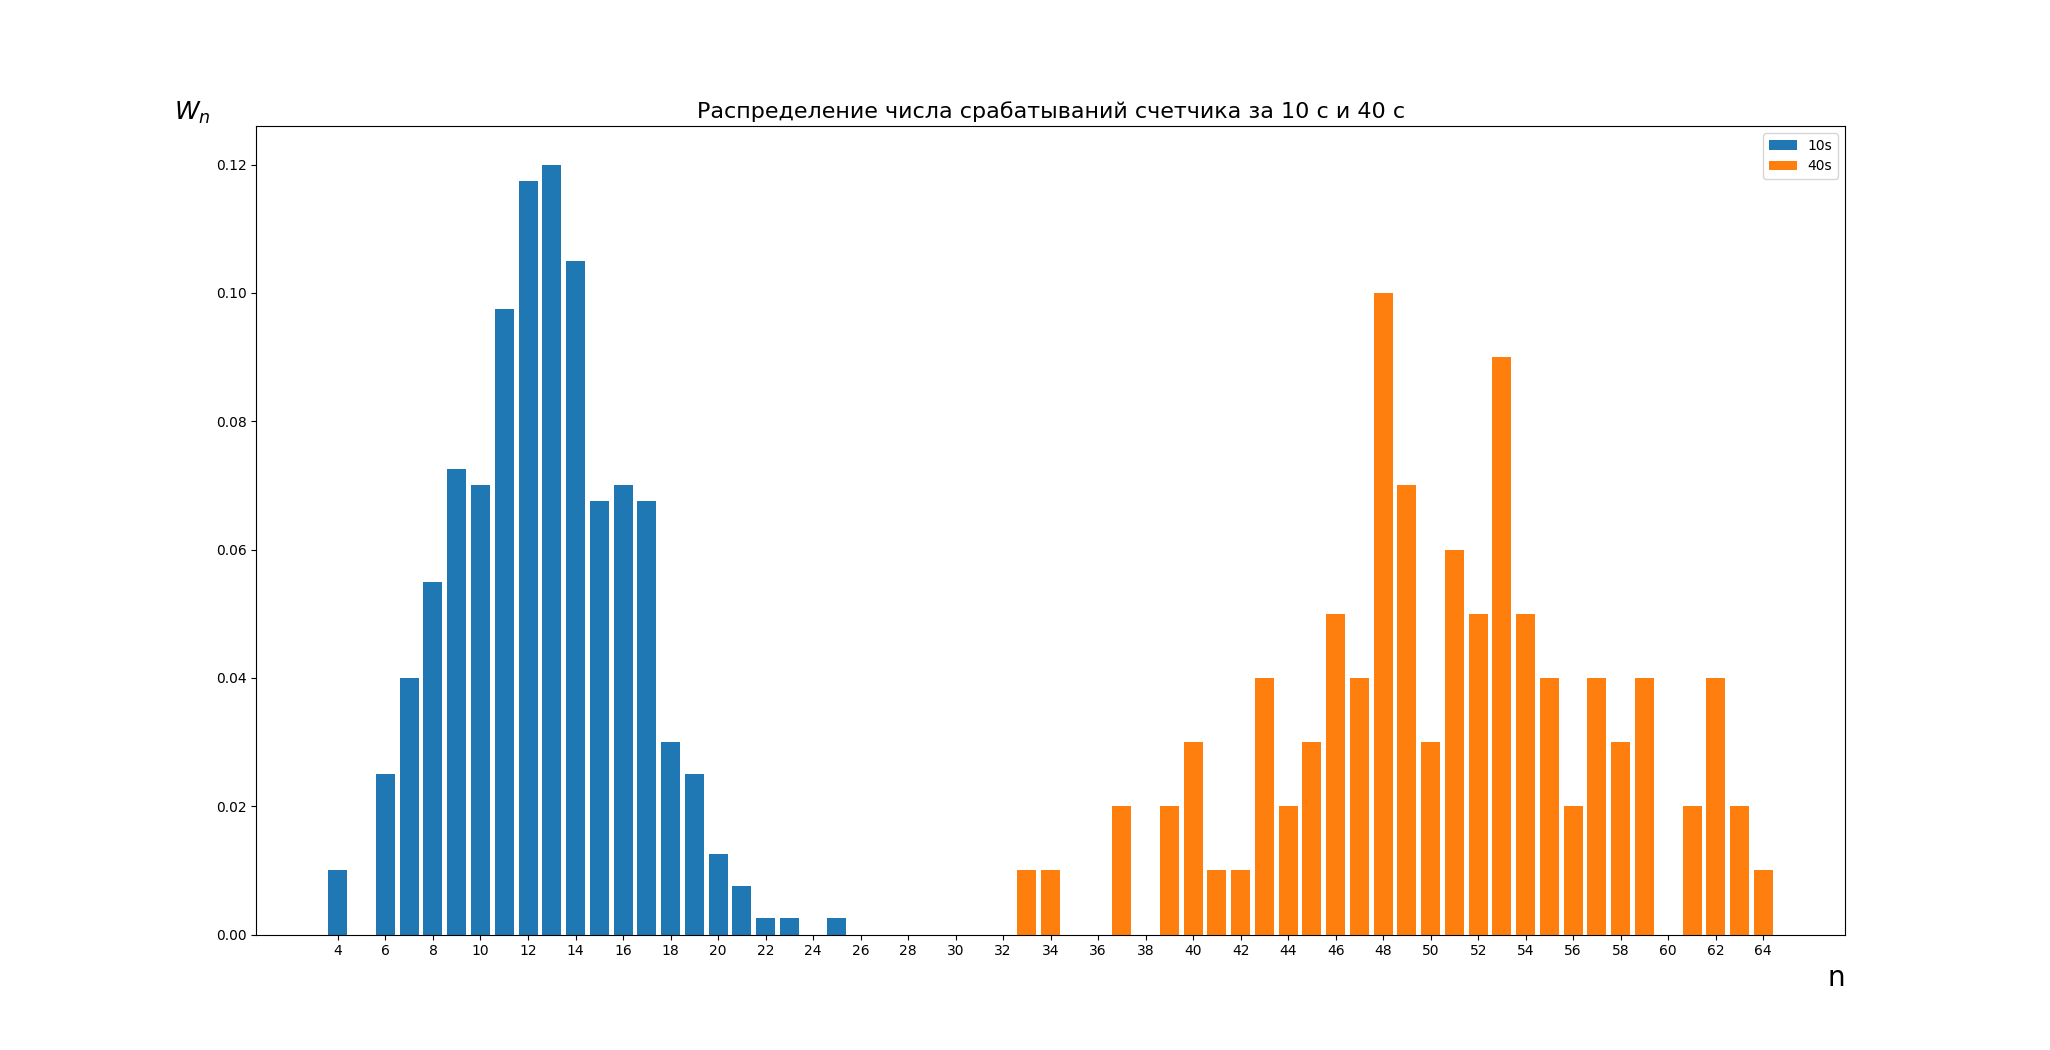
\includegraphics[width=22cm, height=13cm, angle=90]{dist_10_40.png}
\end{center}



Среднее число срабатываний счётчика за 10 с по формуле (1):


\[\overline{n_1} = \frac{5051}{400} = 12,62\]


Среднеквадратичная ошибка отдельного измерения по формуле (2):
\[\sigma_1 = \sqrt{\frac{1}{N}\sum\limits_{i=1}^n (n_i-\overline{n_1})^2} = \sqrt{\frac{5067}{400}} \approx 3,56.\]


Убедимся в справедливости формулы:


\[\sigma_1 \approx \sqrt{\overline{n}_1};\quad 3,56 \approx \sqrt{12,62} = 3,55.\]


Определим долю случаев, когда отклонения от среднего значения не превышают $\sigma_1, 2\sigma_1$
, и сравним с теоретическими оценками:

\begin{center}
    \begin{tabular}{|c|c|c|c|}
        \hline
        Ошибка                   & Число случаев & Доля случаев, \% & Теоретическая оценка \\
        \hline
        $\pm\sigma_1 = \pm3,56$  & $259$         & $65$             & $68$                 \\
        \hline
        $\pm2\sigma_1 = \pm7,12$ & $385$         & $96$             & $95$                 \\
        \hline
    \end{tabular}
\end{center}
\begin{flushright}
    {\scriptsize \textbf{Таблица 5} }
\end{flushright}


Среднее число срабатываний счётчика за 40 с по формуле (1):


\[\overline{n_2} = \frac{5051}{100} = 50,51\]


Среднеквадратичная ошибка отдельного измерения по формуле (2):
\[\sigma_2 = \sqrt{\frac{1}{N}\sum\limits_{i=1}^n (n_i-\overline{n_2})^2} = \sqrt{\frac{4473}{100}} \approx 6,7.\]


Убедимся в справедливости формулы:


\[\sigma_2 \approx \sqrt{\overline{n}_2};\quad 6,7 \approx \sqrt{50,51} = 7,1.\]


Сравним среднеквадратичные ошибки отдельных измерений для двух распределений:
$\overline{n}_1 = 12,62; \sigma_1 = 3,56$ и $\overline{n}_2 = 50,5; \sigma_2 = 7,1$.
Легко видеть, что хотя абсолютное значение $\sigma$ во втором распределении больше,
чем в первом (7,1 > 3,56), относительная полуширина второго распределения меньше:


\[\frac{\sigma_1}{\overline{n}_1}\cdot100\% = \frac{3,56}{12,62}\cdot100\% \approx 28\% \]
\[\frac{\sigma_2}{\overline{n}_2}\cdot100\% = \frac{7,1}{50,51}\cdot100\% \approx 14\% \]

Это также следует из построенных гистограмм.



Определим стандартную ошибку величины $\overline{n_1}$ по формуле (3):


\[\sigma_{\overline{n_1}} = \frac{\sigma_1}{\sqrt{N_1}} = \frac{3,56}{\sqrt{400}} \approx 0,18\]


Найдем относительную ошибку по формуле (4):
\[\epsilon_{\overline{n_1}} = \frac{\sigma_{\overline{n_1}}}{\overline{n_1}}\cdot100\% = \frac{0,18}{12,62}\cdot100\% \approx 1,42\%\]


По равенству $\epsilon_{\overline{n}} = \frac{1}{\sqrt{\overline{n}N}}$ получим:


\[\epsilon_{\overline{n_1}} = \frac{100\%}{\sqrt{12,62\cdot400}} \approx 1,40\%\]


Окончательный результат:
\[n_{t=10c} = \overline{n_1} \pm \sigma_{\overline{n_1}} = 12,62 \pm 0,18\]


Аналогично для $N_2 = 100$ измерений по 40 с:
\[\sigma_{\overline{n_2}} = \frac{7,1}{\sqrt{100}} \approx 0,71\]
\[\epsilon_{\overline{n_2}} = \frac{0,71}{50,51}\cdot100\% \approx 1,41\%\]
\[\epsilon_{\overline{n_2}} = \frac{100\%}{\sqrt{50,51\cdot100}} \approx 1,41\%\]


Окончательный результат:
\[n_{t=40c} = 50,51 \pm 0,71\]



\end{document}
